\subsection{UC5 - Pagamento conto}\label{usecase:5}
\begin{figure}[H]
    \centering
    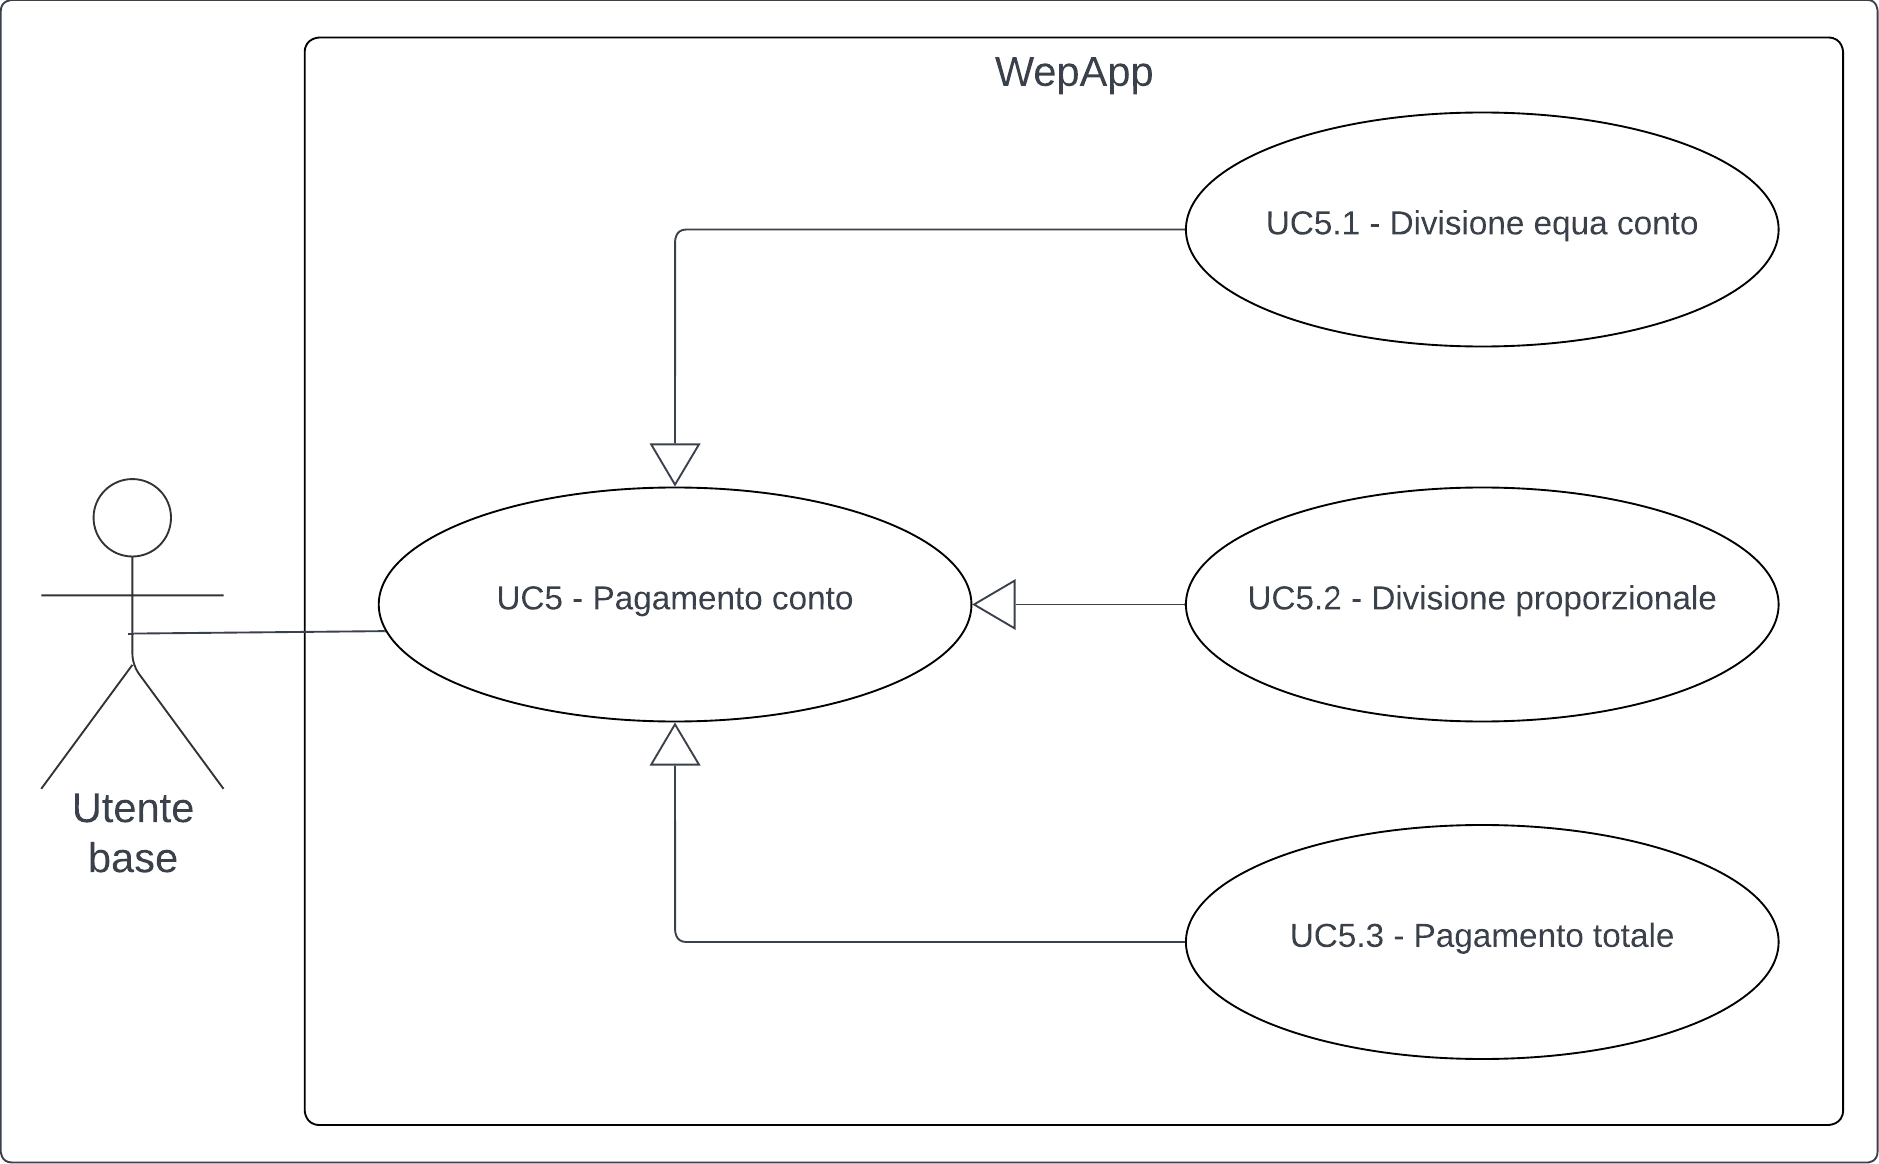
\includegraphics[width=0.7\textwidth]{ucd/UCD5.png}
\end{figure}
\textbf{Attori}:
\begin{itemize}
    \item Utente base autenticato
\end{itemize}
\textbf{Precondizioni}:
\begin{itemize}
    \item L'utente deve aver prenotato un tavolo
    \item L'utente deve aver ordinato (\nameref{usecase:3})
\end{itemize}
\textbf{Postcondizione}:
\begin{itemize}
    \item Il conto del tavolo è stato pagato
\end{itemize}
\textbf{Scenari principali}:
\begin{enumerate}
    \item L'utente può selezionare tra:
    \begin{enumerate}
        \item divisione equa
        \item proporzionale
        \item pagamento totale
    \end{enumerate}
    \item Ogni utente può decidere se pagare solo la sua parte oppure anche le parti di altri utenti
    \item L'amministratore riceve aggiornamenti riguardanti allo stato del conto del tavolo tramite notifiche (push-notification)
\end{enumerate}
\subsubsection{UC5.1 - Divisione equa}\label{usecase:5.1}
\textbf{Attori}:
\begin{itemize}
    \item Utente base autenticato
\end{itemize}
\textbf{Precondizioni}:
\begin{itemize}
    \item L'utente deve aver prenotato un tavolo
    \item L'utente deve aver ordinato (\nameref{usecase:3})
    \item L'utente che ha creato l'ordinazione collaborativa deve aver scelto questo pagamento
\end{itemize}
\textbf{\textit{Postcondizione}_G}:
\begin{itemize}
    \item Il conto del tavolo è stato pagato
\end{itemize}
\textbf{Scenari principali}:
\begin{enumerate}
    \item L'utente paga la sua parte del conto
\end{enumerate}
\subsubsection{UC5.2 - Divisione proporzionale}\label{usecase:5.2}
\textbf{Attori}:
\begin{itemize}
    \item Utente base autenticato
\end{itemize}
\textbf{Precondizioni}:
\begin{itemize}
    \item L'utente deve aver prenotato un tavolo
    \item L'utente deve aver ordinato (\nameref{usecase:3})
    \item L'utente che ha creato l'ordinazione collaborativa deve aver scelto questo pagamento
\end{itemize}
\textbf{Postcondizione}:
\begin{itemize}
    \item Il conto del tavolo è stato pagato
\end{itemize}
\textbf{Scenari principali}:
\begin{enumerate}
    \item L'utente paga la sua parte del conto
\end{enumerate}
\subsubsection{UC5.3 - Pagamento totale}\label{usecase:5.3}
\textbf{Attori}:
\begin{itemize}
    \item Utente base.
\end{itemize}
\textbf{Precondizioni}:
\begin{itemize}
    \item L'utente è connesso al $\textit{Sistema}_G$;
    \item L'utente deve aver ordinato (\nameref{usecase:3});
    \item Il conto del tavolo non è ancora stato pagato parzialmente.
\end{itemize}
\textbf{Postcondizione}:
\begin{itemize}
    \item Il conto del tavolo è stato pagato.
\end{itemize}
\textbf{Scenari principali}:
\begin{enumerate}
    \item L'utente paga per tutto il tavolo.
\end{enumerate}
\newpage